\documentclass[conference]{IEEEtran}
\IEEEoverridecommandlockouts
% The preceding line is only needed to identify funding in the first footnote. If that is unneeded, please comment it out.
\usepackage{cite}
\usepackage{amsmath,amssymb,amsfonts}
\usepackage{algorithmic}
\usepackage{graphicx}
\usepackage{booktabs}
\usepackage{hyperref}
\usepackage{makecell}
\usepackage{glossaries}
\usepackage{textcomp}
\usepackage{xcolor}
\def\BibTeX{{\rm B\kern-.05em{\sc i\kern-.025em b}\kern-.08em
    T\kern-.1667em\lower.7ex\hbox{E}\kern-.125emX}}

\newacronym{batman}{B.A.T.M.A.N.}{Better Approach To Mobile Adhoc Networking}

\newacronym{rtt}{RTT}{Round Trip Time}
\newacronym{arq}{ARQ}{Automatic Repeat-reQuest}
\newacronym{ne}{NE}{Nash Equilibrium}


\begin{document}

\title{A game-theoretical analysis of BATMAN-adv protocol}

\author{\IEEEauthorblockN{Andrea Pittaro}
\IEEEauthorblockA{\textit{Dipartimento di Ingegneria dell'Informazione} \\
Padova, Italy \\
andrea.pittaro@studenti.unipd.it}
\and
\IEEEauthorblockN{Enrico Lovisotto}
\IEEEauthorblockA{\textit{Dipartimento di Ingegneria dell'Informazione} \\
Padova, Italy \\
enrico.lovisotto@studenti.unipd.it}
}

\maketitle

\begin{abstract}
  In this course project we will show how a de-centralized telecommunication network using the popular \gls{batman} protocol can sustain itself without a central control.

  The key point to make this kind of systems feasible and reliable is to reward collaboration and penalize unwanted selfish behaviour: in this case the former consists in forwarding each others packets and the latter in dropping them.

  We will study, simulate and measure performances of a distributed infrastructure in order to empirically evaluate when collaboration is indeed the best strategy for the nodes to pursue, meaning when it is the game \gls{ne}.
\end{abstract}

\section{Introduction}

% - history\\

\gls{batman} was created in 2007 as a mesh networks protocol that allowed users to create network using their devices as nodes that routes traffic and transmit data to the network.

In 2008 it became \gls{batman}-adv breaking the ISO/OSI stack and exploiting knowledge at layer 2 and 3 to efficiently find paths and route the packets arriving to each node. During these years the protocol evolved and in 2011 became officially supported by the Linux Kernel, allowing all PCs to become a node in the network.

Since then, the protocol was widely tested, thanks to the Freifunk initiative, which aims to create a decentralized WiFi network and reaching all Germany.

\begin{figure}[h]
  \centering
  
\includegraphics[width=0.8\linewidth]{figures/logo.pdf}
  \caption{Logo of \gls{batman} project}
  \label{fig:batman_logo}
\end{figure}

\smallskip

% - how does the protocol work: principles

The protocol \gls{batman}-adv creates a network of ad-hoc connections where each node periodically notifies the neighbours of its presence using discovery messages.

Similarly to what is done in traditional distance-vector routing protocols this information is used to build a local table that associates to each known remote destination to the next hop for the packet to cross.

The peculiar feature of the \gls{batman} protocol is that together with this alive messages the nodes will periodically exchange their own local forwarding scheme. The emerging shared knowledge makes the connected entities aware of the global structure of the network and so connections are more reliable and resilient even with mobile and non-persistent users.

In fact, when a node fails other ones can immediately find new paths upon being notified the change of topology.
Conversely, if a node starts acting selfishly, as it disregards forwarding other packets, the network will soon notice its unfair behaviour and will ignore all the packets coming from it.

While for smaller networks such global table can span the whole set of nodes, for bigger ones fixed gateways can be set in order to reach far destinations. This reduces the information required at each node and allows \gls{batman}-adv to run in home routers.

\smallskip

Like every de-centralized protocol, \gls{batman} relies on the contribution of all involved entities in order to sustain itself. Each node plays then a game, choosing between collaboration and egoism: this project aims to assess when the former is preferred to the latter and what kinds of rewards are needed for the players for the wanted behaviour to be the most convenient.

\section{Methodology}

\subsection{Network setup}

In order to study the protocol we decided to take an experimental approach, measuring objective functions of the players in a simulated setting.

As customary in this kind of analysis, a certain number $N$ of nodes is scattered uniformly across a square simulation area of side $L$, as shown in \autoref{fig:nodes}. This allows to change topology simply switching the generator random seed and will be used to validate all our results.

\begin{figure}[h]
  \centering
  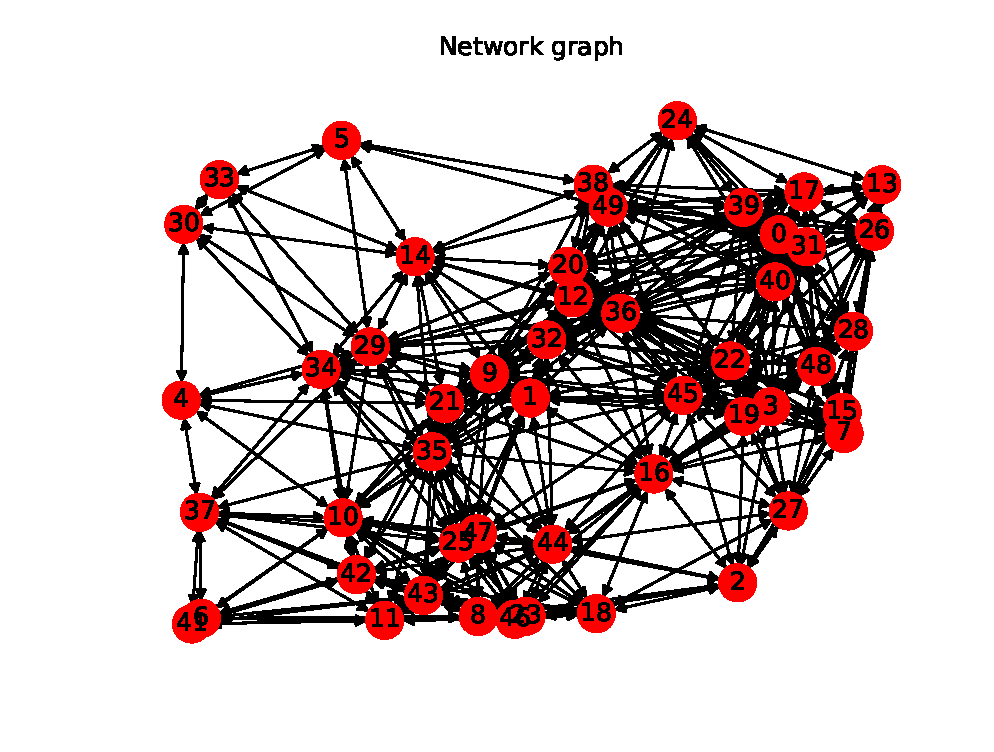
\includegraphics[width=\linewidth]{figures/example_graph}
  \caption{Nodes, labeled by their IP, are connected each other wirelessly.}
  \label{fig:nodes}
\end{figure}

Once placed, each couple of close nodes are linked with wireless fully reliable channels, characterized by a \gls{rtt} and a re-transmission probability $p_r$, both function of the reciprocal distance.

This assumption on the channel characteristics reduces the model complexity while keeping an decent degree of realism, as \gls{arq} strategies are common practice at all protocol stack levels.

\begin{equation}
  \begin{split}
    p_r & = e^{-\frac{d}{D}} \\
    RTT &= 2 \frac{d}{c} + t_{proc}
  \end{split}
\end{equation}
where $c$ is the speed of light, $t_{proc}$ the receiver processing time and $d$ the distance between the two nodes.
\smallskip

Up to this point of network building, nodes are able to communicate but there are still no users for our infrastructure.

Memoryless applications are then randomly and uniformly setup between pairs of points, according to a probability coefficient, called ``app rate''. A fraction of those, defined as ``selfish rate'', will act only for themselves, namely refusing to forward packets from other sources.

User satisfaction, measured in these layers, will be the key to judge the strategy adopted at the \gls{batman} layer.
Regardless of the cooperation or the selfishness of their routing units, which users in fact don't know nor care about, a good node can be easily recognized as the one whose applications are served with an high bitrate to the rest of the network.
To do so, it has to rely to a certain extent on its neighbours, since not all destinations are reachable in a single hop.

\smallskip
Once all details have been defined, the overall communication scenario can be described by messages exchanged in a directed graph made of \gls{batman}, channels and application layers, depicted in \autoref{fig:graph}.

\begin{figure}[h]
  \centering
  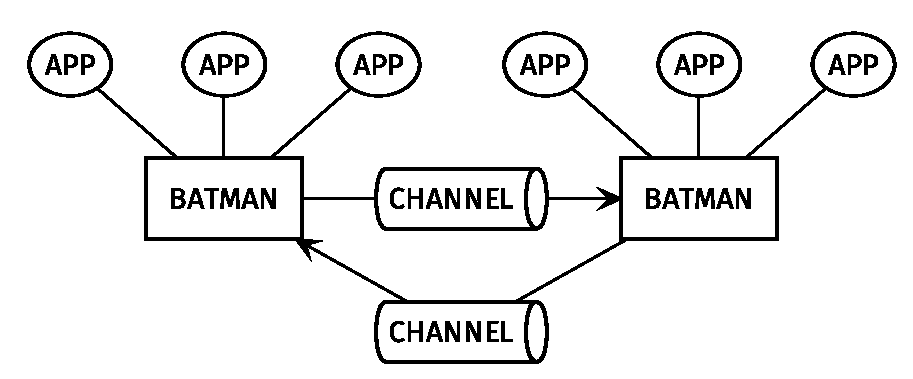
\includegraphics[width=\linewidth]{figures/layers_diagram}
  \caption{Abstract graph spanning all logical components of the network.}
  \label{fig:graph}
\end{figure}

All the parameters of the network relevant for the upcoming study of the objective function are listed in \autoref{tab:params}.

\renewcommand\theadalign{l}

\begin{table}[h]
\resizebox{\linewidth}{!}{%
  \begin{tabular}{@{}lcl@{}}
    \toprule
    Parameter     & Values range & Description                            \\ \midrule
    L             & 100m ÷ 1000m & Network area dimension                 \\
    D             & 100m ÷ 200m  & Distance parameter for $p_r$ and $rtt$           \\
    N             & 10 ÷ 100     & Number of nodes                        \\
    selfish\_rate & 0.01 ÷ 0.1   & Fraction of selfish nodes              \\
    app\_rate     & 0.01 ÷ 0.05  & \thead{Fraction of connected \\couples of nodes} \\ \bottomrule
  \end{tabular}%
}
\vspace{0.1cm}
\caption{Relevant parameters for building the network}
\label{tab:params}
\end{table}

\subsection{Expertiment steps}

As presented above, two different strategies can be chosen by each \gls{batman} layer in order to maximize its objective function: either it can collaborate with others, using part of its bandwidth to forward packets of other sources, or selfishly transmit only its own packets.

As we will show in the upcoming \autoref{sec:results}, if there were no form of punishment, nodes would be encouraged to act selfishly, expecially when others still respects the agreement.

The \gls{batman} protocol is for this reason designed in such a way that the altruistic path is more convenient for the nodes to pursue, pushing the rate of the selfish nodes close to zero. The collaboration will then turn out to be a \gls{ne} for the game played between all the connected entities.

\section{Results} \label{sec:results}

% Network performances between fair and unfair users varying
% - percentage of unfair users
% - requested traffic (number and intensity of apps)
% - channel quality

A naive conception of a distributed routing algorithm could simply rely on the generosity of the nodes, hoping they will share their bandwidth to others.
Since this approach gives no substantial penalty to selfish nodes, they can still profit from the network while making the experience worse for everyone else.

As can be seen in \autoref{fig:no-blame} and in \autoref{fig:no-blame-app-rate}, the two performance lines are very close to each other: no strategy is then  preferable to the other one in terms of profit for the players. For all the plots that we were able to obtain through the simulations, though, we can see that if the rate of the egoistic nodes is less than $0.167$, then a device is slightly encouraged to play his own game, dropping the other player's packets. Over this limit, the nodes are to some degree incentivized to play altruistically as their bitrate is, on a small scale, higher.

\begin{figure}
  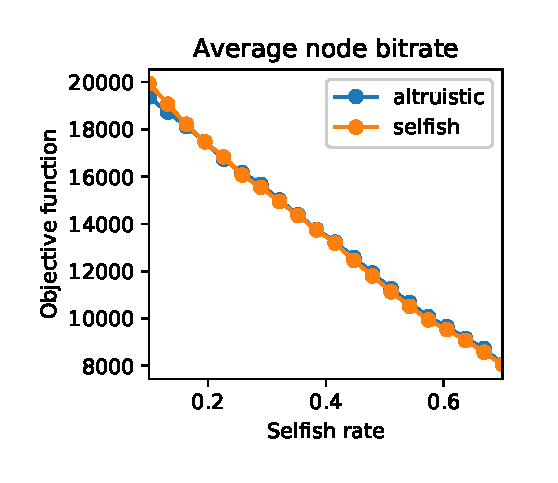
\includegraphics{figures/obj_func_vs_selfish_rate_no_punish.eps}
  \caption{Average bitrate in case no punishment is applied to selfish nodes}
  \label{fig:no-blame}
\end{figure}

\begin{figure}
  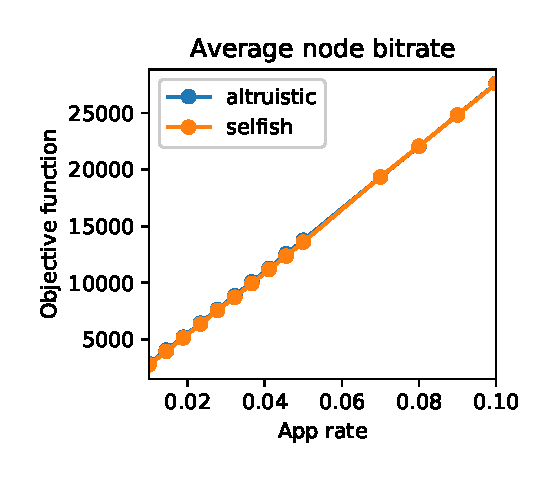
\includegraphics{figures/obj_func_vs_app_rate_no_punish.eps}
  \caption{Average bitrate in case no punishment is applied to selfish nodes}
  \label{fig:no-blame-app-rate}
\end{figure}

This creates a weaker network, since no incentive is given to the altruistic members from the point of view of the objective function.


\section{Conclusion}

\bibliography{report}
% \bibliographystyle{IEEEtran}

\end{document}

%%% Local Variables:
%%% mode: latex
%%% fill-column: 90002000
%%% TeX-master: t
%%% End:
